% (c) 2020 Stefan Antonowicz
% Based off of tex found at https://github.com/ludus-leonis/nipajin
% This file is released under Creative Commons Attribution-NonCommercial-ShareAlike 4.0 International License.
% Please do not apply other licenses one-way.

\renewcommand{\yggMortals}{%
  \mychapter{The Tribes of the Authority}{mortals}
}

\renewcommand{\yggMortalsText}{%

  \flavor{And Kib grew weary of the second game, and raised his hand in the Middle of All, making the sign of Kib, and made Men: out of beasts he made them, and Earth was covered with Men.  \Tilde Lord Dunsany}

  The Tribes of the \TheAuthority, the Mortal races, cover each of the moons of Tartarus - from the tops of Acheron's \myital{Mountains of Madness} to the depths of Styx's \myital{Caliphate of Holes}.  This passing species is pursued by Sish, the Destroyer of Hours, and perish beneath the sign of Mung, the God of All Deaths.  Despite the belief that the children of Kib are just playthings for the Small Gods, they breed and spread prolifically.  Through this cycle of life and death, Order is maintained in the face of Chaos.

 You are marked by the sign of Kib, and blessed with a soul (the \myital{noumenon}, the "thing in itself").  Because you have a soul, you are Hallowed; a member of the Tribes sacred to \TheAuthority.  Hallowed things stand in opposition to Magic - the phenomenon whose rules are bound by Chaos rather than Order.

  Mortals are all of the same species (though their appearance varies greatly!).  Mortal Adventurers divide themselves into four different disciplines called \mybold{Tropes:}


    \mylist {
      \item \mybold{\mylink{The Sellsword}{trope-sellsword}}  \\ The heresy of the Saigoths prophesizes that at the end of things, Mung will set his back against Trehagobol and "...wielding the Sword of Severing which is called Death, shall fight out his last fight with the hound Time, his empty scabbard Sleep clattering loose behind him".  You see the inevitability of Death in everything around you, and seek to be the last standing.  Your Primary Stat is \VIG
      

    }

    \cbreak

    \mylist{


      \item \mybold{\mylink{The Knave}{trope-knave}} \\ In the "Sayings of Limpang-Tung", he vows to "... send jests into the world and a little mirth", and that we should pray to Limpang-Tung "... while Death seems to thee as far away as the purple rim of hills; or sorrow as far off as rain in the blue days of summer".   But ... as we grow old, then it is pointless to pray to Limpang-Tung, for you have become "...part of a scheme that he doth not understand".  You are a thrill-seeker and materialist; you seek to drink down life to the last dregs.  You prefer stealth over violence, but you are capable of much violence if need be.  Your Primary Stat is \DEX 

      \item \mybold{\mylink{The Philosopher}{trope-philosopher}} \\ Eld, first of the high Prophets, told the prophet Imbaun on his initiation that "... we have all looked upwards in the Hall of Night towards the secret of Things, and ever it was dark, and the Secret faint and in an unknown tongue."  As we know, however, Imbaun was to become the prophet of Dorozhand, and was shown "... the paths of Sish stretching far down into future time".  There is always more to know before THE END. You seek to understand the Secret and uncover its power, before you fall beneath the sword of Mung.  Your Primary Stat is \INT
      
      \item \mybold{\mylink{The Mystic}{trope-mystic}}   \\ The eyes of Dorozhand, god of Destiny, have gazed upon the Mystic - they become "... the arrow from the bow of Dorozhand hurled forward at a mark he may not see - to the goal of Dorozhand."  Even the Small Gods fear Dorozhand, for "... they have seen a look in the eyes of Dorozhand that regardeth beyond the gods."  You believe in believing; in fate, kismet, and destiny; that we all have a role to play in the Small God's game at the bedside of \TheAuthority. Your Primary Stat is \FOC
    }
  



  \newpage

  %%%%%%%%%%%%%%%%%%%%%%%%%%%%%%%%%%%%%%%%%%%%%%%%%%%%%%%%%%%%%%%%%%%%%%
  %%%%  SELLSWORDS %%%%%%%%%%%%%%%%%%%%%%%%%%%%%%%%%%%%%%%%%%%%%%%%%%%%%
  %%%%%%%%%%%%%%%%%%%%%%%%%%%%%%%%%%%%%%%%%%%%%%%%%%%%%%%%%%%%%%%%%%%%%%

  \mysection{The Sellsword}{trope-sellsword}

  \flavor{
    How heavy this axe \\
    Burden carried from birth \\
    Wrought in Stygian visions \\
    By the gods of the earth \Tilde The Sword, "How Heavy this Axe"
  }

  \mysubsection{Base Stats}{sellsword-base-stats}

  \mybullet{ 
    \item  Sellswords have a d10 \FLESH
    \item  Sellswords have Fortitude
    \item  Sellswords have a d4 Deed Die
  }


  \myhighlight{Fortitude}{sellsword-fortitude}
  
  You add your \LVL to any \RO or \RB attempt that includes your \VIG die.  

  \myhighlight{The Deed Die}{sellsword-deed-die} 

  The Deed Die is a \UD whose result can be applied to any of your Fight checks. Roll the Deed Die and add its result to your Fight roll; if you hit, also add the result to your damage (applied \mybold{after} the die explodes, if applicable).  You can roll your Deed Die \myital{after} your Fight check is rolled (it doesn't have to be at the same time), but you can only roll it once per Moment.  Don't forget that this is a \UD, so it moves \DCDOWN if you roll a 1 or a 2.  You get a Deed Die back when you take a \mylink{Vacation}{civilization-vacation}.

    \begin{center}
  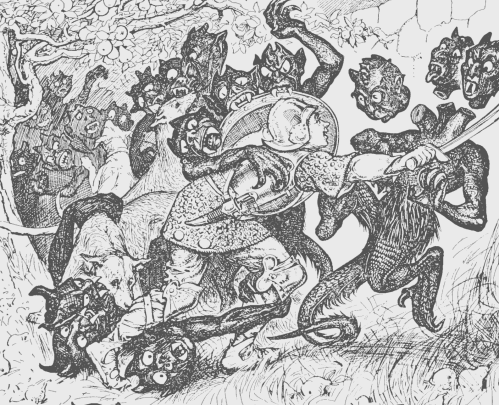
\includegraphics[scale=.45]{Sellsword_1}
  \end{center}



  \cbreak


  \mysubsection{Creation}{sellsword-creation}

  \callout{
    \mynumlist {
      \item Move any of your core Skills \DCUP
      \item Move any of your core Saves \DCUP
      \item Pick \mybold{three} \mylink{Virtues}{sellsword-virtues} from the list below.  You can only pick each Virtue once.
      \item Pick \mybold{one} \mylink{Complication}{sellsword-complications} from the list below (or make up your own with the Arbiter!)
      \item Write down your Starting Gear
    }
  }


    \mytable{X}{
      \thead{\mysubsection{Virtues}{sellsword-virtues}} \\
    }{ 
      Blademaster \\
      Duelist \\
      Huntsman \\
      Intangibles \\
      Lethal \\
      My Father's Sword \\
      Second Skin \\
      Three Kills Per Stroke \\
      Tougher Than a Coffin Nail \\
      Veteran \\
    }

    \myhighlight{Blademaster}{sellsword-virtue-blademaster}

    Two handed weapons count as one Significant Item instead of two. You also add your \LVL to damage (applied \mybold{after} the die explodes, if applicable)

    \myhighlight{Duelist}{sellsword-virtue-duelist}

    You start the game with two Fast weapons of your choice (including the Knave's Sword).  You can use the Florentine Mighty Deed regardless of your \DEX

    \myhighlight{Huntsman}{sellsword-virtue-huntsman}

    You start the game with Light Armor and a Strongbow with a Quiver of Arrows (d10 \UD)

    \myhighlight{Intangibles}{sellsword-virtue-intangibles}

    You may move two different Intangible Stats of your choice \DCUP.  Describe to the Arbiter why these Intangible Stats are better than average.

    \myhighlight{Lethal}{sellsword-virtue-lethal}

    If you roll \MAX damage for your weapon, the die explodes i.e. you roll again and add the second roll to the first.  If you roll \MAX damage again, the roll continues.  This roll has to be a \myital{natural} (not modified) roll (though some powers and abilities can change a natural roll).  Modifiers to damage are added or subtracted  \mybold{after}  the die explodes (including Deed Die).  Note that this means you can't \mylink{Crit}{combat-crits-and-fumbles} since your last roll is never technically the \MAX. 

    \example{Charse the Lethal attacks a goblin with a Shortsword (d6).  He makes his Fight check and hits, and rolls a 6 for damage. He rolls again and rolls another 6.  He rolls a 3rd time and rolls a 4.  He deals 16 points of damage(!) [6+6+4] and the goblin is reduced to a fine pink mist.}


    \myhighlight{My Father's Sword}{sellsword-virtue-fathers-sword}

    You start the game with a Hard Brawl weapon of your choice.  With this weapon \mybold{only} your Fight \RO is +4, your damage explodes as if you had the Trait \mylink{Lethal}{sellsword-virtue-lethal}, and you cannot be Disarmed. If you lose this weapon, you lose the abilities that go with it.  You have to describe to the Arbiter what makes this weapon unique.

    \myhighlight{Second Skin}{sellsword-virtue-second-skin}

    Your armor doesn't count as a Significant Item.  You can repair 1 \UD of your Armor when you take a \mylink{Breather}{combat-resting-breather}, 
    up to its \MAX \UD.   You start the game with a suit of Light or Medium Armor.  The Armor should look unique; describe what it looks like to the Arbiter.

    \myhighlight{Three Kills Per Stroke}{sellsword-virtue-three-kills}
    
    Treat any Brawl weapon you use as if it had Cleave.

    \myhighlight{Tougher Than a Coffin Nail}{sellsword-virtue-coffin-nail}

    Immediately:
    \mylist {
        \item Raise any of your Saves \DCUP (this is in addition to your initial Save \DCUP);
        \item Raise your \DEATH to start at \mybold{Tough, d6}
        \item Add +2 Flesh
    }

    Every time you gain a level:  roll your \VIG.  If the result of your roll is greater than your current Flesh, replace your Flesh with that result.  You can make this roll at any time during Vacation.

    \example{Charse the Tough currently has 12 Flesh, and hits level 2.  He chooses to advance his \VIG to d12, then opts to roll for his new Flesh.  He rolls a d12 and adds his \LVL (since he's rolling his Primary Stat), getting a 13.  Nice.  He now has 13 Flesh)}

    \myhighlight{Veteran}{sellsword-virtue-veteran}

    You have some experience with a prior \mylink{Band}{the-band}.  You start with d6+1 Grit.  Tell the Arbiter the name of your old \mylink{Band}{the-band}, and what happened to them.




    \mytable{X}{
      \thead{\mysubsection{Complications}{sellsword-complications}} \\
    }{
      Alcoholic \\
      Cheap Tricks \\
      The Cimmerian \\
      Credo \\
      Filthy \\
      Hippophobia \\
      Honorable \\
      Mortal Enemy \\
      Pit Fighter \\
      Sins of the Father \\
    }

    \myhighlight{Alcoholic}{sellsword-complication-alcoholic}

    You are addicted to alcohol.  Whenever you take a Breather, you have to take a drink or you heal no Grit.  \RS your \VIG when you do - if you Fail, you gain 1 point of \mylink{Drunk}{effect-drunk}. 

    When you take a Bivouac, you must roll a \UD for an alcoholic beverage, or you gain none of the beneficial effects. \RS your \VIG at the end of the Bivouac - if you fail, you are \mylink{Hung Over}{effect-hung-over}


    \myhighlight{Cheap Tricks}{sellsword-cheap-tricks}

    You do not like or trust magic, \mylink{Philosophers}{trope-philosopher}, or the unnatural (including \mylink{The Unseelie}{unseelie}).  The degree to which you feel this way is up to you.  Let the Arbiter know why.

    \myhighlight{The Cimmerian}{sellsword-complication-cimmerian}

    Your appearance is so outlandish even educated and well-traveled people will stop to stare at you. People can pick you easily out of a crowd, and your reputation precedes you.

    \myhighlight{Credo}{sellsword-complication-credo}
  
    You must make a vow - a short, specific, personal statement that you will not forget. For example, "I will protect my friend Johann" or "I will never harm an unarmed person".  You must follow this vow to the best of your ability

    \myhighlight{Filthy}{sellsword-complication-filthy}

    You refuse to bathe except under the most dire circumstances.  Your general hygiene is horrible.  You can never use your Presence to charm someone (intimidate is a different story), and if you're downwind from Monsters it might affect your ability to surprise them.

    \myhighlight{Hippophobia}{sellsword-complication-hippophobia}

    You are afraid of horses and mules.  You refuse to ride one (riding in a cart is OK).


    \myhighlight{Honorable}{sellsword-complication-honorable}

    You refuse payment for good deeds, rescue the helpless, and refuse to fight unarmed foes (within reason, of course).  

    \myhighlight{Mortal Enemy}{sellsword-complication-mortal-enemy}

    You have a mortal enemy, someone powerful who has done you significant wrong.  This enemy should be substantially more powerful than you.  You are driven by your revenge against this mortal enemy. Tell the Arbiter who they are, and why they are your enemy.

    \myhighlight{Pit Fighter}{sellsword-complication-pit-fighter}

    You strongly believe that combat should take place between two people face-to-face.  You won't use Shoot weapons, and you'll never throw a Throw weapon at a target.

    \myhighlight{Sins of the Father}{sellsword-complication-sins-father}

    Your parent (alive or dead) is infamous.  If people ever discover that you are their child, they will have significant negative reactions.  At the Arbiter's complete discretion you will encounter various assassins, sellswords, and kidnappers who have figured out who you are, and want to do you harm.  Tell the Arbiter a bit about this parent.


  \mysubsection{Starting Gear}{sellsword-starting-gear}

  \mybullet {
    \item 2 iron pieces; 
    \item a backpack containing a worn bedroll;
    \item d4 \UD of personal provisions;
    \item a stained and patched waterproof cloak;
    \item a pitted shield, rusty helmet, and sharpened spear
    \item one pick OR 3 rolls on the \mylink{Random Items}{appendixb-random-items} table in Appendix B;
  }   


    \mysubsection{Examples}{sellsword-examples}

    \myhighlight{The Old Campaigner}{sellsword-soldier}

    \example{Travel, Veteran, Second Skin, My Father's Sword, Credo}

    \myhighlight{The Barbarian}{sellsword-barbarian}

    \example{Bushcraft, Tougher Than a Coffin Nail, Three Kills Per Stroke, Lethal, The Cimmerian}

    \myhighlight{The Sword Saint}{sellsword-sword-saint}

    \example{Listen, Blademaster, Lethal, Duelist, Alcoholic} 
    
    \myhighlight{The Ranger}{sellsword-ranger}

    \example{Bushcraft, Veteran, Lethal, Huntsman, Honorable}


    \newpage

  %%%%%%%%%%%%%%%%%%%%%%%%%%%%%%%%%%%%%%%%%%%%%%%%%%%%%%%%%%%%%%%%%%%%%%
  %%%%  KNAVES %%%%%%%%%%%%%%%%%%%%%%%%%%%%%%%%%%%%%%%%%%%%%%%%%%%%%%%%%
  %%%%%%%%%%%%%%%%%%%%%%%%%%%%%%%%%%%%%%%%%%%%%%%%%%%%%%%%%%%%%%%%%%%%%%

  \mysection{The Knave}{trope-knave}

  \flavor{Fortune and glory, kid.  Fortune and glory. \Tilde Indiana Jones}

  \mysubsection{Base Stats}{knave-base-stats}

  \mybullet{ 
    \item  Knaves have a d8 \FLESH
    \item  Knaves have Puissance
    \item  Knaves have a d4 Luck Die
  }


  \myhighlight{Puissance}{knave-puissance}

  Knaves add their \LVL to any \RO or \RB attempt they're trying that includes their \DEX.  

  \myhighlight{Luck Dice}{knave-luck-die}

  Knaves have a Luck Die - a unique \UD whose result can be applied to any \RO or \RB try that includes \DEX.  Roll the Luck Die and add its result to your \RO or \RB check.  You can only roll your Luck Die once per \RO or \RB


  \mysubsection{Creation}{knave-creation}

  \callout{
    \mynumlist {
      \item Move any of your core Skills \DCUP
      \item Move any of your core Saves \DCUP
      \item Pick \mybold{three} \mylink{Virtues}{knave-virtues} from the list below.  You can only pick each Virtue once.
      \item Pick \mybold{one} \mylink{Complication}{knave-complications} from the list below (or make up your own with the Arbiter!)
      \item Write down your Starting Gear
    }
  }



    \mytable{X}{
      \thead{\mysubsection{Virtues}{knave-virtues}} \\
    }{
      Deadeye \\
      Duelist \\
      Guilded \\
      Inked \\
      Intangibles \\
      Mummy's Curse \\
      Whispers of Anne Bonny  \\
      Whispers of Br'er Rabbit  \\
      Whispers of Sun Wukong  \\
      Whispers of The Bride  \\
    }


    \myhighlight{Deadeye}{knave-virtue-deadeye}

    Requires you to know the \mylink{Whispers of The Bride}{knave-virtue-the-bride}.  If you're hidden and take an Action to Aim, you can \mylink{Murder}{knave-murder} with a Throw or Shoot weapon.

    \myhighlight{Duelist}{knave-virtue-duelist}

    You start the game with two Fast weapons of your choice (including the Knave's Sword).  You can use the Florentine Mighty Deed regardless of your \DEX

    \myhighlight{Guilded}{knave-virtue-guilded}

    You are the ex member of a Thieves' Guild. In addition to your starting gear, pick 3 items from the following list:
    \dashedbox {
      \mybullet {
        \item a suit of Light armor;
        \item a set of two silver daggers;
        \item a Bow and quiver of arrows (d10 \UD);
        \item 5 picks from the \mylink{Adventuring Gear}{gear-adventuring} table;
        \item a pouch of 3 gems (roll on the \mylink{Gems table}{appendixb-random-treasure} in Appendix B);
        \item d4 \UD of a Narcotic of your choice;
        \item a Fetish with d4 \UD of any spell you choose;
        \item d4 \UD of an Iron Toxin    
      }
    }

    Tell the Arbiter the name of your ex-Guild, and why you left ...    


    \myhighlight{Inked}{knave-virtue-inked}

    You start the game with all of the following Tattoos:  Dagger, Torch, Compass, and Rope\footnote


    \myhighlight{Intangibles}{knave-virtue-intangibles}

    You may move two different Intangible Stats of your choice \DCUP.  Describe to the Arbiter why these Intangible Stats are better than average.

    \myhighlight{Mummy's Curse}{knave-virtue-mummys-curse}

    You're immune to the effects of cursed or supernatural items you carry as long as you intend to sell them.  If you use the item or gain any benefit from it, you suffer the negative effects    

    \myhighlight{Whispers of Anne Bonny}{knave-virtue-ann-bonny}

    You know the whispers that help you climb walls, disguise yourself, forge documents, swing from chandeliers, and fight with two weapons.  See the section on \mylink{Whispers}{knave-whispers} below for more details.

    \myhighlight{Whispers of Br'er Rabbit}{knave-virtue-brer-rabbit}

    You know the whispers that help you pick pockets, escape prisons, perform sleight-of-hand, and cast spells from Fetishes.  See the section on \mylink{Whispers}{knave-whispers} below for more details.

    \myhighlight{Whispers of Sun Wukong}{knave-virtue-sun-wukong}

    You know the whispers to hide things on your person, find and disarm traps, and open locks.  See the section on \mylink{Whispers}{knave-whispers} below for more details.

    \myhighlight{Whispers of The Bride}{knave-virtue-the-bride}

    You know the whispers that help you move silently, hide in shadows, apply poisons, and murder your victims.  See the section on \mylink{Whispers}{knave-whispers} below for more details.


    \begin{center}
      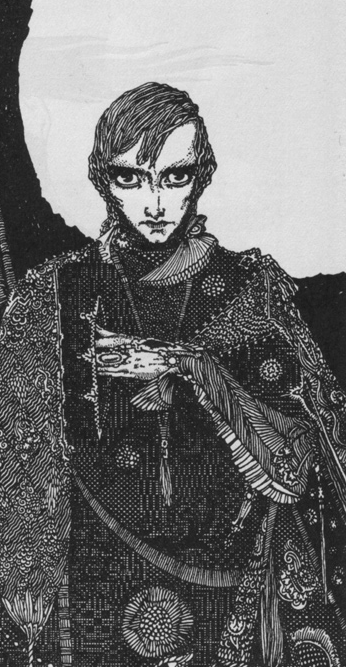
\includegraphics[width=0.48\textwidth]{Knave}
    \end{center}


  \newpage

    \mysubsection{Whispers}{knave-whispers}

    \example {
        \RB: \KNAVE (optional: \PLUS \LUCK - Difficulty) vs. Difficulty
    } 

    Whispers are the disciplines, incantations, hedge magic, illusion, sleight-of-hand, and minor telepathy that constitute the \mybold{Left Hand Path}.  Passed down through instruction, ancient books, and word-of-mouth, Whispers allow you to trick reality into doing what you want.

    Your skill in each of the four Whispers is represented by one of the following \STATIC die, called a \KNAVE

    \mytable{X r}{
      \thead{Rank} & \thead{\KNAVE} \\
    }{
      Apprentice & d4 \STATIC \\
      Footpad & d6 \STATIC \\
      Sharper & d8 \STATIC \\
      Master & d10 \STATIC \\
    }

    You may buy additional ranks in a Whisper when you \mylink{advance in level}{advancement-leveling}

    You must be unarmored or wearing \mylink{Light Armor}{gear-armor} to use your Whispers.  You cannot perform Whispers while using a shield.   Using a Whisper in combat is a \mylink{Basic Maneuver}{combat-basic-maneuver}.  Finally, Whispers require verbalization; you must be able to speak in order to use a Whisper (a common punishment for thieves is to cut out their tongues).

    Rolling your \KNAVE should only be required by the Arbiter if the difference between success and failure would be interesting, or when the attempt shouldn't be an automatic success.

    If the Arbiter decides the roll is required, she will set a Difficulty (a number between 1 and 9) for the roll (details on difficulty are found in the Arbiter's section on \mylink{Knavery}{arbiter-knave}).  \RB than this number using your \KNAVE (ties go to the Adventurer!)

    You may use your \LUCK to affect your \KNAVE roll, but \mybold{the Difficulty is subtracted from your Luck roll}.  You cannot go below 0 in this way.  Again, see the section on \mylink{Knavery}{arbiter-knave} in the Arbiter's section to get a sense of your odds of success.



    \example {
      Flink Lighthand is 3rd level and a Footpad in the Whispers of Sun Wukong (so he has d6 \KNAVE and d6 \LUCK), and he's robbing a crypt.  Creeping down a hallway he peeks through the broken door of an antechamber, and sees the glint of gold at the far end.  Flink's sixth-sense is tingling though, and he asks the Arbiter if he sees any traps in here.  The Arbiter knows there's a cunning poisoned spear trap in the room and assigns a difficulty of 4/2 to it (4 to find it and 2 to disarm it).  Flink rolls his \KNAVE and gets a 4 - he smells a whiff of tarantula venom in the air, and the large flagstone just inside the door seems to shimmer for a moment.  Bending close to the flagstone that would release the trap, Flink whispers to it and asks it to lock in place.  He rolls again ... and gets a 1!  Thinking quickly, Flink rolls his \LUCK and rolls a 4.  He has to subtract the 2 difficulty from this roll and gets a total of 3 (1 + (4 - 2)).  Lucky break, he's able to recover, and the trap mechanism disarms.
    }


    \myhighlight{Whispers of Anne Bonny}{knave-whisper-ann-bonny}

    Also known as The Swashbuckler, Anne Bonny's instructions show the ways to scale impenetrable fortresses, icy cliffs, and wizard's towers; swing from ropes and vines; disguise yourself to escape patrolling soldiers or to get past armed guards; and forge documents to start wars or gain access to restricted areas. If you are a student of the Whispers of Anne Bonny, a Knave's Sword gains both the Rend and Cleave ability in your capable hands.

    \myhighlight{Whispers of Br'er Rabbit}{knave-whisper-brer-rabbit}

    Br'er Rabbit (The Curious) knows a thing or two about tight squeezes.  His Whispers can help you remove items from pockets without anyone seeing; perform sleight-of-hand, ventriloquism, and distraction to befuddle your marks; escape from ropes and manacles; and cast spells from Fetishes.  If you are a student of the Whispers of Br'er Rabbit, you can turn Invisible (as the spell) once per Session.

    When casting spells from a Fetish, you roll your \KNAVE for the Whispers of Br'er Rabbit instead of Blood Dice.  You can add the result of a \LUCK to this roll as well. The difficulty of reading a spell off a specific Fetish is up to the Arbiter, but the difficulty should default to 0.   

    \myhighlight{Whispers of Sun Wukong}{knave-whisper-sun-wukong}

    Sun Wukong is known as The Thief.  His teachings show the secret ways of hiding things on your person so they are difficult to find; uncovering and understanding the mechanisms of traps, snares, and Inscribed Sigils and chide them into disarming themselves; and opening locked chests, doors, and prisons.  If you are a student of the Whispers of Sun Wukong, you can make a sack, bag, or satchel into a Hammerspace Bag.

    \example {
      The \mybold{Hammerspace Bag} can contain up to 12 Significant Items.  Searching for a Significant Item is a 1-in-(number of items) chance of finding it per Moment i.e. if you have 6 Significant Items in the bag, you have a 1-in-6 chance of pulling it out in a Moment.  You can pull out Insignificant Items stored in the bag immediately.  The effect is permanent until you die, but you can only have one Hammerspace Bag at a time.  If you die, all of the contents of the bag are immediately ejected
    }


    \myhighlight{Whispers of The Bride}{knave-whisper-the-bride}

    The Bride is known by many names, none of them spoken aloud:  Lady Death, the Banshee, the Viper, etc.  Education in the Whispers of the Bride teaches you the mental tricks, hypnotism, and observation necessary to sneak past (or behind) people without them noticing you, to silence the clink of coins in your pocket and the sound of your breath and heartbeat. In addition, the Bride teaches you the finer points of committing Murder, provided you get \mylink{the Drop}{combat-surprise} . If you are a student of the Whispers of the Bride, you do not need to make \DEX checks for handling Toxins or Acids.

    \cbreak

    \myhighlight{Murder}{knave-murder}

    If you get \mylink{The Drop}{combat-surprise} on someone, you can attempt a Murder.  Murder can only be performed at Close range with a Shortsword, Dagger, Club, or Hand Axe.  Make a standard Fight \RO; if you hit, pick \mybold{one} of the following attacks:

    \dashedbox {
      \mybullet {
        \item \mybold{Cautious:}  You automatically \mylink{Crit}{combat-crits-and-fumbles} (do maximum damage + \LVL).  Any weapon.
        \item \mybold{Reckless:}  You do 3d6 damage.  Any weapon.
        \item \mybold{Bloody:}  You roll damage normally, but the Monster is also Bleeding. Stabbing only.
        \item \mybold{Waylaying:}  You can either roll damage and the Monster is Woozy, or do no damage and the Monster must Save or be Knocked Out.  Bashing only.
      }
    }

   Murder is a Combat Action, so it can't be combined with other Combat Actions (like Florentine). Damage bypasses any Armor or Soak, if applicable (you slip the blade between the Monster's scales / plate mail / chink in carapace). Once you commit a Murder, you no longer have the Drop unless you're able to get out of sight again. Note that Monsters who are Amorphous or immune to surprise cannot be Murdered. 

  \newpage

  \mybold{Murder cont. (example)}

  \example {
    Deego Foxears (3rd Level Knave and student of The Bride) and Stalwart Hamhands (3rd Level Sellsword) come around the corner and surprise a clutch of three Ghouls and a necromancer standing at an altar.  The ghouls are Close and the necromancer is Nearby.  The Arbiter rules the ghouls and necromancer are surprised, so Flink has The Drop.  He tries his Fight \RO and succeeds.  He's armed with a Knave Sword and opts to attack "Cautiously".  He deals 11 damage (8 for the sword + \LVL) and stabs a ghoul through the heart before it can react. Stalwart steps up behind him and guts another ghoul with his polearm.  The single remaining ghouls rolls morale and (somehow) decides to stay and fight.

    ~\\

    Deego and Stalwart roll Init - Deego rolls well over 20, Stalwart less so (he's wearing plate mail).  Deego takes the opportunity to duck into the shadows to try to get the Drop on the necromancer. The Arbiter gives the difficulty a 3 (2 for the ghoul's \HD; an extra 1 because the ghoul is Close and aware Deego's there, but he's mostly focussed on the huge armored guy with a polearm; and no modifier for the necromancer, who's completely absorbed in his ritual). Deego rolls his d6 and gets a 5, and slips out of view.  The Ghoul attacks Stalwart and hits, but Stalwart is able to absorb the damage with his Grit.  The necromancer seems to be trying to finish his ritual and doesn't make a move.  It's Stalwart and Deego's turn; Deego takes another Tactical Maneuver and moves Nearby (right behind the necromancer), while Stalwart engages the remaining ghoul.  Depending on how Init goes the next Moment, Deego will be able to take a Combat Action, and hopefully stop the wizard from releasing some eldritch horror ...
  }

 \cbreak


    \mytable{X}{
      \thead{\mysubsection{Complications}{knave-complications}} \\
    }{
      Arch-nemesis \\
      Cursed \\
      Expensive Tastes \\
      Honor Among Thieves \\      
      Outstanding Contract \\
      Pacifist \\
      Pandemonium \\
      Religious \\
      Remorseless \\
      Superstitious \\
    }

    \myhighlight{Arch-Nemesis}{knave-complication-archnemesis}
    
    You have an arch-nemesis who always seems to be a step ahead of you when it comes to obtaining artifacts. Tell the Arbiter a little bit about them.

    \myhighlight{Cursed}{knave-complication-cursed}

    Probably should have left that amulet alone.  Roll on the TK TK TK Curse table - you start the game under that curse.  Tell the Arbiter how you acquired this curse.

    \myhighlight{Expensive Tastes}{knave-complication-tastes}

    You have exquisite and deviant tastes in the fine things in life. It costs you twice as much to take a \mylink{Vacation}{civilization-vacation}; the money spent is still applied to your experience.

    \myhighlight{Honor Among Thieves}{knave-complication-honor}

    You're a professional, and you appreciate other professionals.  You'll always give a hand to a fellow Knave even if that might inconvenience your \mylink{Band}{the-band}.

    \myhighlight{Outstanding Contract}{knave-complication-contract}

    There's an outstanding contract on your head, revenge for something you did.  Tell the Arbiter who and why they want to kill you.

    \myhighlight{Pacifist}{knave-complication-pacifist}

    You won't ever start a fight (including stabbing someone unawares in the back).  You have no problems fighting once a fight is joined, however.  

    \newpage 

    \myhighlight{Pandemonium}{knave-complication-pandemonium}

    You spend money as fast as you can make it, steal from the rich to give to the poor, and thrive in chaos.  You aren't motivated by anything material; you want anarchy, discord, and confusion.    

    \myhighlight{Religious}{knave-complication-religious}

    You are very religious (secretly or not).  You don't worship a specific Small God necessarily, but you have enormous respect for Mystics, the Authority, and the Thrones.  You won't steal anything from a church or temple; priest of priestess - regardless of the Small God.


    \myhighlight{Remorseless}{knave-complication-remorseless}

    You feel nothing when you take a life or cause pain, but you suffer from \mylink{Night Terrors}{madness-night-terrors}.  This affliction can never be cured.


    \myhighlight{Superstitious}{knave-complication-superstitious}

    You are extremely superstitious (and believe this superstition has kept you alive up until now).  You fear the Malocchio and prefer the company of Pooka whenever possible.  You won't steal from the dead, or take anything from tombs or graves.


    \mysubsection{Starting Gear}{knave-starting-gear}


    \mybullet {
      \item 10 iron pieces; 
      \item a set of belt pouches;
      \item d4 \UD of personal provisions;
      \item two daggers OR 1 short sword;
      \item one pick OR 3 rolls on the \mylink{Random Items}{appendixb-random-items} table in Appendix B;
    }

    \cbreak

    \mysubsection{Examples}{knave-examples}

    \myhighlight{The Bandit}{knave-bandit}

    \example{Travel, Whispers of The Bride, Guild's Gift, Inked, Pandemonium}
    
    \myhighlight{The Assassin}{knave-assassin}

    \example{Listen, Whispers of The Bride, Whispers of Br'er Rabbit, Deadeye, Religious}
   
    \myhighlight{The Buccaneer}{knave-buccaneer}

    \example{Salt, Whispers of Anne Bonny, Duelist, Intangibles (Talent), Expensive Tastes}
   
    \myhighlight{The Archaeologist}{knave-archaeologist}

    \example{Lore, Mummy's Curse, Whispers of Br'er Rabbit, Whispers of Sun Wukong, Pacifist}




    \newpage

  %%%%%%%%%%%%%%%%%%%%%%%%%%%%%%%%%%%%%%%%%%%%%%%%%%%%%%%%%%%%%%%%%%%%%%
  %%%%  Philosopher %%%%%%%%%%%%%%%%%%%%%%%%%%%%%%%%%%%%%%%%%%%%%%%%%%%%%%%
  %%%%%%%%%%%%%%%%%%%%%%%%%%%%%%%%%%%%%%%%%%%%%%%%%%%%%%%%%%%%%%%%%%%%%%

  \mysection{The Philosopher}{trope-philosopher}

  \flavor{Holy Diver!  You've been down too long in the midnight sea … \Tilde Dio, "Holy Diver"}


  \mysubsection{Base Stats}{philosopher-base-stats}

  \mybullet{ 
    \item  Philosophers have a d6 \FLESH
    \item  Philosophers have Genius
    \item  Philosophers can Research
  }

  \myhighlight{Genius}{philosopher-genius}

  Philosophers add their \LVL to any \RO or \RB attempt they're trying that includes their \INT 

  \myhighlight{Research}{philosopher-research}

  Philosophers can spend Research when they are taking a \mylink{Vacation}{civilization-vacation}.  

  \mysubsection{Creation}{philosopher-creation}

  \callout{
    \mynumlist {
      \item Move any of your core Skills \DCUP
      \item Move any of your core Saves \DCUP
      \item Pick \mybold{three} \mylink{Virtues}{philosopher-virtues} from the list below.  You can only pick each Virtue once.
      \item Pick \mybold{one} \mylink{Complication}{philosopher-complications} from the list below (or make up your own with the Arbiter!)
      \item Write down your Starting Gear
    }
  }

  \begin{center}
  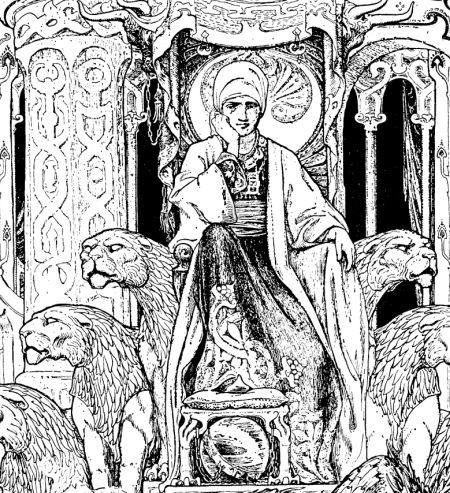
\includegraphics[scale=.45]{Philosopher}
  \end{center}

    \mytable{X}{
      \thead{\mysubsection{Virtues}{philosopher-virtues}} \\
    }{
      College \\
      The Crux of Blood \\
      The Crux of Knowledge \\
      Intangibles \\
      Leechcraft  \\
      Research: Chymistry \\
      Research: Inscription  \\
      Research: Medicinals  \\
      Staff Magic \\
      Wizardry \\
    }


    \myhighlight{College}{philosopher-virtue-college}

    You received an education and some equipment from one of the many Philosopher's Colleges that dot the major cities of Acheron.  You start with \mybold{three} of the following:


    \dashedbox {
      \mybullet {
      \item a Polearm;
      \item a Grimore with 5 spells of your choice (these spells can be added to a Grimoire if you already have one);
      \item a set of two silver daggers;
      \item a Fetish with d4 \UD of any spell you choose;
      \item a suit of Light or Medium armor (incompatible with Wizardry);
      \item 5 picks from the \mylink{Adventuring Gear}{gear-adventuring} table;
      \item a pouch of 3 gems (roll on the \mylink{Gems table}{appendixb-random-treasure} in Appendix B);
      \item d4 \UD of a Narcotic of your choice 
    }}

  \myhighlight{The Crux of Blood}{philosopher-virtue-blood}

  You push yourself to the edge of madness and reason, riding the warp and weft of the fabric of existence to master the arcane words that are gibbered and shrieked by the creatures beyond the Void.  They seek blood in payment - the sap of  Ygg, the brine of the Six Seas, the fire inside the calderas that felled Atlantis.  Blood is Life, and they desire it more than anything.  Blood aids great sorcery. Blood is Power.  

  You gain 1 d6 Blood \POOL; you can use this \POOL to evoke Wizardry.  You have a single spell written inside of your skull. \footnotemark 

  \myhighlight{The Crux of Knowledge}{philosopher-virtue-knowledge}

  Magic exists.  Undeniably.  To say otherwise would be to defy what we know.  But those who try to control \myital{arcana} are buffeted by it, controlled by it, consumed by it.  Slain by it.  Science though - that is \myital{our} creation.  It exists to serve - humble, obedient, and aloof.  Few have the discipline to seduce it; it takes a lifetime of dedication, a lifetime of asking "why?" over and over again and knowing that there will be no end to the question.  "Why?" will reverberate in the heavens when the last star winks out.  "Why?" is a quest, a calling.  It drives us to travel the heights and depths, tame the riches of the world, cheat death and defy Chance and spit in the face of Luck.  When you walk the path of "Why?", you follow in the footsteps of Gods.

  You gain 1 d8 Knowledge \STATIC; you can use this \STATIC to practice Leechcraft.\footnotemark[\value{footnote}]

  \myhighlight{Intangibles}{philosopher-virtue-intangibles}

    You may move two different Intangible Stats of your choice \DCUP.  Describe to the Arbiter why these Intangible Stats are better than average.

  \myhighlight{Leechcraft}{philosopher-virtue-leechcraft}

  Requires the Crux of Knowledge.  Combat medicine, sewing wounds, and alleviating pain.  Get them back in the fight!
 
  \myhighlight{Research: Chymistry}{philosopher-virtue-chymistry}

  Put a stopper in death.  Create potions and salves, toxins and acids. Gain 1 point of Research.\footnotemark[\value{footnote}]

  \myhighlight{Research: Inscription}{philosopher-virtue-inscription}
  
  Klaatu barada nikto! Read and write magical texts and inscriptions, divine words of power, and research True Names. Gain 1 point of Research.\footnotemark[\value{footnote}]

  \myhighlight{Research: Medicinals}{philosopher-virtue-medicinals}

  Cure diseases, addictions, wounds, and madness through the power of science. Gain 1 point of Research.\footnotemark[\value{footnote}]

  \myhighlight{Staff Magic}{philosopher-virtue-staff-magic}

  \myital{His staff! I told you to take the Wizard's staff!}  Create a Magic Staff or Caduceus\footnotemark[\value{footnote}] to assist your Wizardry or Leechcraft

  \myhighlight{Wizardry}{philosopher-virtue-wizardry}

  Requires the Crux of Blood. Plunge headfirst into the arcane tempest and tap its power.  Choosing this Virtue grants you a Grimoire with 3 random spells in it, and allows you to harvest spell components from defeated foes\footnotemark[\value{footnote}]

  \footnotetext{See the Bell, Book, and Candle PDF}
  \setcounter{footnote}{0}

    \mytable{X}{
      \thead{\mysubsection{Complications}{philosopher-complications}} \\
    }{
      Bibliophile \\
      It is I - Balthazar the Breathtaking! \\
      Logical \\
      Morbid \\
      Mysophobia \\
      Necronomicon \\
      One More Page \\
      Out of Shape \\
      Whoops! \\
      Transcendental Research \\
    }


  \myhighlight{Bibliophile}{philosopher-bibliophile}          

  You really, really love books. If given the choice between a share of treasure and books you haven't read, you will opt for the books every time.  You will look to build a library and hire porters to carry spare books around for you.  The books you covet must be unusual or educational (practically, this means grimoires or books that teach or augment Skills).  You must have at least 3 Significant Items worth of books with you at all times.  Tell the Arbiter about your favorite book.

  \myhighlight{It is I - Balthazar the Breathtaking!}{philosopher-complication-arrogance}

  There's your typical run-of-the-mill arrogance - braggarts, blowhards, and boasters - and then there's you.  Your arrogance is on a whole other level.  You won't tolerate any other Philosophers in your Band.  You accept no masters and believe in no law but your own. To "the Man", you are an appalling spectacle, and should be put in your place (or in the ground) before you harm anyone else.

  \myhighlight{Logical}{philosopher-logical}

  You are devoid of any emotion.  People call you cold, distant, or calculating.  When faced with a decision or dilemma, you will always opt for the logical, unemotional response.

  \myhighlight{Morbid}{philosopher-morbid}

  You require corpses - fresher the better - to perform Research (Chymistry, Inscription, or Medicinals).  You'll need at least 1 fresh corpse if you want to Research during a \mylink{Vacation}{civilization-vacation}. 

  \cbreak\bump

  \myhighlight{Mysophobia}{philosopher-mysophobia}

  You have an morbid fear of "contamination".  You wear a mask and gloves that you rarely take off, insist on cleanliness whenever possible, keep your clothing and gear in neat order, and bathe often. Tell the Arbiter how you got this way.

  \myhighlight{Necronomicon}{philosopher-necronomicon}

  You are in possession of a forbidden tome, text, or fetish.  It's taught you everything you need to know and (quite possibly) made you slightly insane.  All of your Research (Chymistry, Inscription, or Medicinals) has to start with this book; practically, you have to \RS: Sanity whenever you spend any Research.  Tell the Arbiter what this book is, and how you got it.

  \myhighlight{One More Page}{philosopher-one-more-page}

  During a Bivouac, you can't seem to stop reading, writing, drawing, or hypothesizing.  You must make a \RS \FOC check when you take a Bivouac, in addition to your Provision roll.  If you Fail (roll a 1 or a 2), you don't get any of the benefits of having rested.

 \myhighlight{Out of Shape}{philosopher-out-of-shape}

  You're a little (ok, a lot) out of shape.  One of your Significant Item slots is taken up by your excess weight, and you aren't able to run for longer than Minutes.

  \myhighlight{Transcendental Research}{philosopher-transcendental-research}

  You require narcotics to do Research (Chymistry, Inscription, or Medicinals).  Pick a \mylink{Narcotic}{gear-narcotics}; you must roll a \UD of this Narcotic any time you spend Research during a \mylink{Vacation}{civilization-vacation}.


  \myhighlight{Whoops!}{philosopher-whoops}

  An experiment or spell went awry some time in your past.  Roll twice on the Mishaps table in Bell, Book, \& Candle.

\newpage

  \mysubsection{Starting Gear}{philosopher-starting-gear}


\mybullet {
    \item a bedroll; 
    \item a book hanger;
    \item a pipe and d4 \UD of tobacco;
    \item a quarterstaff;
    \item one pick OR 3 rolls on the \mylink{Random Items}{appendixb-random-items} table in Appendix B;
  }


\cbreak


\mysubsection{Examples}{philosopher-examples}

\myhighlight{The Doctor}{philosopher-doctor}

\example{Lore, Crux of Knowledge, Leechcraft, Research:Medicinals, Morbid}

\myhighlight{The Sorcerer}{philosopher-sorcerer}

\example{Lore, Crux of Blood, Wizardry, Research:Inscription, Whoops!}

\myhighlight{The Alchemist}{philosopher-alchemist}

\example{Eyeball, Research: Inscription, Research: Chymistry, College, Transcendental Research}




  \newpage

  %%%%%%%%%%%%%%%%%%%%%%%%%%%%%%%%%%%%%%%%%%%%%%%%%%%%%%%%%%%%%%%%%%%%%%
  %%%%  MYSTIC %%%%%%%%%%%%%%%%%%%%%%%%%%%%%%%%%%%%%%%%%%%%%%%%%%%%%%%%
  %%%%%%%%%%%%%%%%%%%%%%%%%%%%%%%%%%%%%%%%%%%%%%%%%%%%%%%%%%%%%%%%%%%%%%  

  \mysection{The Mystic}{trope-mystic}

  \flavor{Creedsmen roll out across the dying dawn - Sacred Israel holy mountain Zion - Sun beams down on to the sandsea reigns - Caravan migrates through deep sandscape - Lungsmen unearth the creed of Hasheeshian - Procession of the weed-priests to cross the sands - Desert legion smoke-covenant is complete - Herb bales re-tied on to backs of beasts - Arise arise arise - The Son of the God of Israel - Jordan river flows on evermore - Bathe in glow of sunlight's beating rays - They feel the serpent's standard rule our day \Tilde Sleep, "Dopesmoker"}

    \begin{center}
  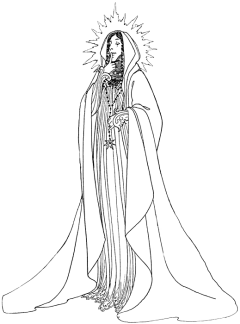
\includegraphics[scale=.38]{Mystic}
  \end{center}

  \cbreak


  \mysubsection{Base Stats}{mystic-base-stats}

  \mybullet{ 
    \item  Mystics have a d4 \FLESH
    \item  Mystics are Contemplative    
  }

  \myhighlight{Contemplative}{mystic-contemplative}

  Mystics add their \LVL to any \RO or \RB attempt they're trying that includes their \FOC


  \mysubsection{Creation}{mystic-creation}


  \callout{
    \mynumlist {
      \item Move any of your core Skills \DCUP
      \item Move any of your core Saves \DCUP
      \item Pick \mybold{three} \mylink{Virtues}{mystic-virtues} from the list below.  You can only pick each Virtue once.
      \item Pick \mybold{one} \mylink{Complication}{mystic-complications} from the list below (or make up your own with the Arbiter!)
      \item Write down your Starting Gear
    }
  }



    \mytable{X}{
      \thead{\mysubsection{Virtues}{mystic-virtues}} \\
    }{
      Aura \\
      Charms  \\
      Cunning \\
      The Crux of Mojo \\
      The Crux of Faith \\
      The Gift of Grace \\
      Initiate \\
      Intangibles \\
      Liturgies \\
      Necromancy \\
    }


    \myhighlight{Aura}{mystic-virtue-armor}

    You use your Mojo as both a shield and a weapon.  You treat your Mojo as an Armor \UD in Combat; additionally, you shape your Mojo into a weapon of your choice.  You use your \FOC for Fighting and deal Mojo \UD in damage. The same Mojo \UD is used for both Armor and Weapon.  Wearing armor, a shield, or a helmet or using a weapon interferes with your Aura - you can't use your Aura if you're so armed or attired.

    Describe to the Aribiter what the Armor and Weapon look like.

    \myhighlight{Charms}{mystic-virtue-charms}

    You may cast Charms and cantrips at will\footnotemark

    \myhighlight{Cunning}{mystic-virtue-cunning}

    You gain 2 Cunning, allowing you to practice Occultism.  Your fate is also now guided by the waxing and waning of the moons and planets.  You gain a Familiar.\footnotemark[\value{footnote}]

    \myhighlight{The Crux of Mojo}{mystic-virtue-mojo}

    True magic is not written. It is passed down, mother to daughter, since the very beginning.  It is richly colored, deeply echoing, singing in the rivers and whispering through the leaves.  The Philosopher seeks it in the Void or inside some book or rattling around at the edges of madness, but that is false magic, waiting to betray.  True magic is the pulling of a baby from the womb, knitting bones and purging poisons, reading the entrails and speaking with the crickets and seeing the patterns in the smokes. This is not some power that is beyond mortal reckoning, but a power that is here for anyone - from king to mudlark - to harness for weal or woe.

    You gain 1 d8 Mojo \UD; you can use this \UD to protect yourself, perform Occult rituals, and practice Necromancy.\footnotemark

    \myhighlight{The Crux of Faith}{mystic-virtue-faith}
  
    Only the most foolhardy or insane pray to the Authority, \TheAuthority, the God of Having Done.  None may pray to Him lest he wake from his dream and call down THE END; it is too great a risk. Rather, all our prayers must be rendered unto  the gods that He created, the Small Gods, the Gods of Doing - and they shall protect us, and guide us, and give us power over men in their honor.  For if the Authority should wake, and we cease to be, what is it all for?  The only true power is Faith.  In a universe that is a dream, and where nothing matters, then the greatest thing you can do is Believe.

    You gain 2 d4 Faith \POOL and your \MAX Faith is 5. You can use Faith to perform Miracles, and to perform the \mylink{Liturgies}{mystic-virtue-liturgies} of one of the Small Gods.\footnotemark[\value{footnote}]


    \myhighlight{The Gift of Grace}{mystic-virtue-grace}

    The Authority whispered seven words before lying down to sleep, words whose echoes still vibrate through the cosmos.  The echoes of the echoes of these words can still be heard to those who listen.  

    You gain 1 d4 Grace \UD; you can use this Grace to perform the Seven Sacraments (Bless, Heal, Loaves and Fishes, Walk on Water, Consecrate, Curse the Unhallowed, Meditation).\footnotemark[\value{footnote}]


    \myhighlight{Initiate}{mystic-virtue-initiate}

    You are no stranger to the trials and travails of life; you have accumulated some gear to keep you alive longer.  You can pick \mybold{three} of the following:

    \mylist {
      \item a Fast weapon of your choice;
      \item a Hard weapon of your choice;
      \item a Magical athame (treat as a normal dagger that can strike creatures only affected by magic) 
      \item a suit of Light armor;
      \item a suit of Medium armor;
      \item 5 picks from the \mylink{Adventuring Gear}{gear-adventuring} table;
      \item a pouch of 3 gems (roll on the \mylink{Gems table}{appendixb-random-treasure} in Appendix B);
      \item d4 \UD of 3 different Narcotics; or d10 \UD of one;
      \item a \mylink{Mule}{gear-transport};
      \item 3 rumors from the Arbiter about your first adventure.  These rumors can be opaque but they must be true.
    }


    \myhighlight{Intangibles}{mystic-virtue-intangibles}

    You may move two different Intangible Stats of your choice \DCUP.  Describe to the Arbiter why these Intangible Stats are better than average.

    \myhighlight{Liturgies}{mystic-virtue-liturgies}

    Requires the Crux of Faith.  Choose a Throne, and a Small God who sits beneath it (this can be a Small God that's listed, or a Small God of your choosing).  You learn the Liturgy of the Novitiates of that Small God, and can perform it using the Crux of Faith.  You also gain a Holy Symbol with 1 Faith \POOL "inside" of it.\footnotemark[\value{footnote}]

    \myhighlight{Necromancy}{mystic-virtue-necromancy}

    Requires the Crux of Mojo.  You can question and command the dead.\footnotemark[\value{footnote}]




  \mytable{X}{
    \thead{\mysubsection{Complications}{mystic-complications}} \\
  }{
    Animal Lover \\
    Burn the Witch! \\
    Cat's Eyes \\
    Heretic \\
    Imma Smoke It \\
    My Name is Earl \\
    Otherworldly \\
    Transubstantiation \\
    The Unseelie \\
    Vow of Poverty 
  }

  \myhighlight{Animal Lover}{mystic-animal-lover}

  You love all kinds of animals; you refuse to ride beasts of burden (including being pulled in a cart by them), eat meat, or suffer the mistreatment of an animal (does not apply to animals that are actively trying to kill you).

  \myhighlight{Burn the Witch!}{mystic-complication-witch}
  
  Any time you stay in a Tiny Civilization, you run the risk of being accused of witchcraft.  If you stay in a Tiny thorp, dorf, etc. roll 2d6 - on a 2 (snake-eyes) you're accosted for poisoning the well water / getting the farmer's daughter pregnant (your gender is irrelevant) / making the chickens sick, etc.  However, if you roll a 12, you'll be called on to do something important - deliver a baby, heal someone's fever, etc.

  \myhighlight{Cat's Eyes}{mystic-cats-eyes}

  Through some mishap, you have the eyes of a cat.  They unfortunately don't allow you to see very well in the dark (treat as if you were holding a candle, probably enough to read by but not much else).  They glow in the dark, however, making it difficult (though creepy) to sneak up on the unwary

  \myhighlight{Heretic}{mystic-complication-heretic}

  Name a Small God.  This God is heretical to your belief; its followers must be slain, its temples desecrated, and its name forgotten

  \myhighlight{Imma Smoke It}{mystic-imma-smoke-it}

  You're constantly looking for new and better ways to transcend the mortal plane and see into the heart of the universe i.e. to get high.  If there's a weird mushroom, you're going to try it.  Some kind of slime, put it in your pipe and see what happens.  I hope you've decided to bump your Toxins Save.

  \myhighlight{My Name is Earl}{mystic-name-is-earl}

  You have set out on the path of the Mystic thanks to the help and sacrifice of another.  You can never repay this debt, so you must pay forward kindness whenever possible.  Tell the Arbiter what this debt is, and who it is to.

  \myhighlight{Otherworldly}{mystic-otherworldly}

  You are eerie, uncanny, and unreal.  You don't cast a reflection, and your footprints appear backwards.  Common folk want nothing to do with you; the more powerful persons you meet treat you at arm's length if not with downright disdain.  

  \myhighlight{Transubstantiation}{mystic-transubstantiation}

  Requires Cunning or the Crux of Faith.  Your Occultism and Miracles are fueled by your own flesh and blood - not a lot, anywhere between a few drops and a goblet-full; a small slice off a limb to a fingertip's worth.  The effects of using your own flesh and blood in this way can have ... interesting effects ... at the complete discretion of the Arbiter.

  \myhighlight{The Unseelie}{mystic-unseelie}

  The Unseelie are Unhallowed, anathema in the eyes of the Authority.  The Unseelie deserve your contempt at best, to be burned at the stake at worst.

  Alternately, the Unseelie are cursed and alone.  The deserve your pity and understanding, and to be protected from the infantile fears and hatreds of Mortals.

  \myhighlight{Vow of Poverty}{mystic-vow-of-poverty}

  You have taken a vow of poverty.  You will never possess more money than you need to live a basic existence; you live as humbly as you possibly can.  You still insist on your full share of treasure, but you will donate it or give it away.  The donation must be anonymous, and you cannot gain Faith in this way (though you can gain XP if you spend this money during a \mylink{Vacation}{civilization-vacation}).

  \mysubsection{Starting Gear}{mystic-starting-gear}

  \mybullet {
    \item a quarterstaff and dagger; 
    \item 2 iron pieces;
    \item a pipe and d4 \UD of tobacco;
    \item 3 picks OR 5 rolls on the \mylink{Random Items}{appendixb-random-items} table in Appendix B;
  } 

  \cbreak
  

  \mysubsection{Examples}{mystic-examples}

  \myhighlight{The Wandering Monk}{mystic-example-wandering-monk}

  \example{Bushcraft, Crux of Mojo, Aura, Seven Sacraments, Animal Lover}

  \myhighlight{The Shaman}{mystic-example-shaman}

  \example{Lore, Crux of Mojo, Aura, Necromancy, Otherworldly}

  \myhighlight{The Witch}{mystic-example-witch}

  \example{Lore, Crux of Mojo, Charms, Cunning, Burn the Witch!}

  \myhighlight{The Pilgrim}{mystic-example-pilgrim}

  \example{Travel, Crux of Faith, Seven Sacraments, Liturgies, The Unseelie}

  \footnotetext{See the Bell, Book, and Candle PDF}
  \setcounter{footnote}{0}
   
} %end
